\chapter{Description du système}

Le but principal du système est de pouvoir récupérer des informations relatives à plusieurs sportifs puis de centraliser les données. Par la suite une application mobile exploitera ses informations pour montrer à l’utilisateur la situation globale de la course au moyen d’une carte.

Pour se faire le système est composé de trois éléments principaux :
\begin{itemize}
\item Un capteur contenant une antenne GPS, une sonde rythme cardiaque et un accéléromètre
\item Un gateway ou passerelle qui récupère les données transmises par le ou les capteurs
\item Une application mobile qui est chargée d’analyser et d’afficher les informations de chaque sportif
\end{itemize}

Les sportifs seront équipés d’un capteur qui permettra l’acquisition des différentes données, à intervalles réguliers les capteurs vont transmettre les informations récoltées, une passerelle est ensuite chargée de récupérer les données puis de les stocker dans une base de données relationnelles.

Une ou plusieurs passerelles seront placées le long du parcours afin de pouvoir garantir une récupération optimale des données des capteurs et ainsi limiter les zones d’ombres ce qui péjorerait l’efficacité du système. C’est principalement la topologie de l’endroit où se tient la course qui déterminera le nombre de passerelles qui devront être employé, cependant le nombre de participant sera également un facteur à prendre en compte. Dans le cadre du travail de Bachelor et à cause des contraintes de temps qui y sont relatives, une seule passerelle ainsi qu’un capteur seront assemblés, la démonstration du système se tiendra donc dans un endroit permettant l’utilisation d’une seule passerelle dans des conditions permettant le fonctionnement optimal du système avec un seul coureur.

Une fois que les données des coureurs ont été reçues, traitées et stockées, l’application mobile récupère les informations depuis la base de données et les analyse pour pouvoir les restituer au spectateur au moyen d’une carte géographique ainsi que de tableaux de statistiques.

Le système de capteur utilisera la technologie LoRa afin de transmettre les informations récoltées à la passerelle. C’est un protocole de télécommunication radio à bas-débit destiné à des objets connectés à basse consommation électrique et de petite taille. Un des avantages principaux du protocole LoRa pour le genre d’application visé par ce projet de diplôme est qu’il ne nécessite pas d’autorisation spéciale pour son utilisation car la bande de fréquence qu’il utilise fait partie du domaine libre. Ces bandes de fréquences peuvent être utilisées dans un espace réduit pour des applications diverses dans les domaines industrielles, scientifiques, médicales domestiques ou similaires. Elle permet aussi l'envoie de messages à des distance entre 2 km dans un milieu urbain voir jusqu’à 15 km dans un environnement dépourvu d’obstacle grâce à des mécanismes qui rendent les messages résistants aux interférences externes. De plus il ne nécessite aucun surcoût, à contrario du GSM (Global System for Mobile Communications) par exemple, qui requiert une carte SIM pour pouvoir communiquer sur le réseau. On comprend tout de suite l’avantage du LoRa par rapport au GSM si l’on pense au fait que pour un seul événement en théorie plusieurs centaines de capteurs pourraient être utilisé en même temps. 

Une fois que les données ont été traitées et stockées dans la base de données, l’application mobile doit pouvoir les récupérer. Pour le prototype la base de données sera directement hébergée sur la passerelle, celle-ci doit être connectée à un réseau qui doit également être accessible à travers l’application mobile. Pour se faire, la solution la plus simple est de connecter la passerelle au réseau en utilisant soit une connexion de type WiFi ou alors de type Ethernet standard. Ceci permettra ensuite, à condition que le téléphone portable ou la tablette exécutant l’application mobile soit connecté à ce même réseau, à l’application de faire des requêtes à destination de la base de données. Pour des raisons de logistiques, il se peut qu’une connexion de type 3G ou 4G soit plus appropriée si par exemple il n’est pas possible à la passerelle de se connecter par d’autres moyens à la base de données. Cet aspect ne sera pas abordé dans le cadre du travail de diplôme mais cela peut être une voie d’évolution pour la suite.

La figure ~\ref{fig:elem_system} montre la situation d’ensemble et les interactions des éléments du système.

\begin{figure}[htb]
\centering 
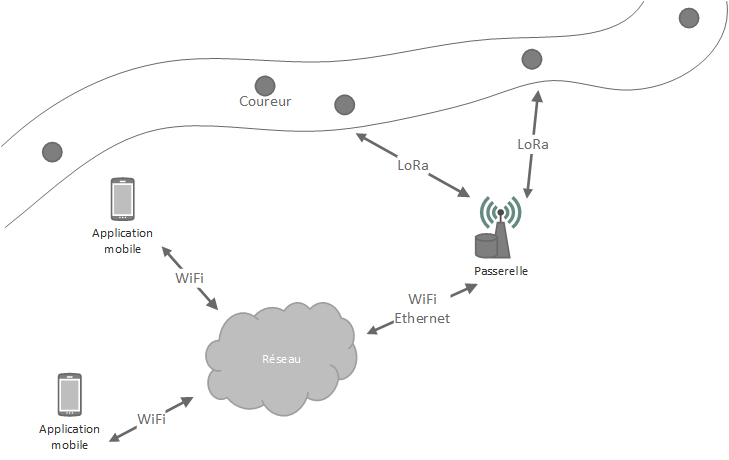
\includegraphics[width=1\columnwidth]{../images/schema_systeme_projet.png} 
\caption[ElemSystem]{Schéma de description du système}
\label{fig:elem_system}
\end{figure}

\section{Fréquence de transmission}

La fréquence de transmission des données est un des points critique du projet. En effet elle doit être assez élevée pour permettre au système de fonctionner correctement, c’est-à-dire de garantir une réactivité suffisante pour rendre l’application agréable à l’utilisation, mais elle doit également respecter les contraintes liées à la technologie LoRa.

Dans le cadre du projet et parmi les paramètres qui vont être enregistrés par le capteur, l’élément qui va permettre de dimensionner la fréquence de transmission est la position GPS du coureur car c’est cette position qui doit être transmise assez souvent pour permettre une mise à jour fréquente de la carte géographique par l’application mobile. D’un point de vu temporel, les autres éléments, c’est-à-dire le rythme cardiaque et la cadence de pas son moins critique.

Afin définir la fréquence de transmission, il est nécessaire de définir la fréquence d’acquisition de la position GPS afin d’obtenir le résultat voulu. L’être humain le plus rapide au monde, Usain Bolt, peut atteindre la vitesse de \SI{44.72}{\km\per\hour}, bien sur cette vitesse ne peut être maintenue que sur une courte distance de sprint. Ce projet est destiné à des courses à pied plus longue, de fond, c’est-à-dire à partir de \SI{5}{\km} de distance. Chez les hommes le record de cette distance est détenu par l’Ethiopien Kenenisa Bekele avec un temps de 12 :37.35 minutes ce qui correspond à une vitesse moyenne d’environ \SI{23.8}{\km\per\hour} et chez les femmes par l’Ethiopienne Tirunesh Dibaba avec un temps de 14 :11.15 minutes c’est-à-dire environ \SI{21.1}{\km\per\hour}. \cite{iaff_all_time_top_list}

Si l’on part du principe qu’un coureur très rapide peu atteindre une vitesse de \SI{20}{\km\per\hour} ou environ \SI{5.5}{\m\per\s}, une fréquence d’acquisition de la position GPS toutes les 30 secondes, ce qui correspond à une distance d’environ \SI{165}{\m}, doit permettre de pouvoir afficher le parcours du coureur sur la carte avec assez de précision. 

Il faudra encore approfondir cette question durant la réalisation du projet pour vérifier si cette valeur suffit ou s’il est nécessaire d’augmenter la fréquence d’acquisition. Une analyse devra également être menée pour définir si cette fréquence est compatible avec le duty cycle imposé par l’utilisation de la bande de fréquence ISM. Le duty cycle définit le temps pendant lequel un élément est autorisé à transmettre des données en utilisant cette bande de fréquence, c’est une contrainte que tous les éléments doivent respecter et qui dépend de la quantité de donnée à transférer ainsi que du débit.
